\chapter{Articles}

\section{Abstract}

The most interesting researches and probably the ones that will be used are :
\begin{itemize}
	\item \citeref{sub:sec:res1}
	\item \citeref{sub:sec:res2}
	\item \citeref{sub:sec:res4}
	\item \citeref{sub:sec:res5}
	\item \citeref{sub:sec:res6}
\end{itemize}

\section{MRI-based DL/ML}

\subsection{\href{https://www.sciencedirect.com/science/article/pii/S187887502032698X\#abssec0015}{Convolutional Neural Networks for Pediatric Refractory Epilepsy Classification Using Resting-State Functional Magnetic Resonance Imaging (May 2021)}}
\label{sub:sec:res1}

Study made to evaluate the performance of CNN in "the classification of patients with paediatric epilepsy from healthy control"

To modify CNNs, some parameters were manually changed, such as: 3 hyperparameters, learning rate, dropout rate and regularization, and number of epoch.

To evaluate them ($\sim$4000 models), the model with the highest sensitivity was kept.

Could be used to test other programs.

\subsubsection{Methods}

Full explanations of each step in the paper, figure summing up here: \citeref{fig:res1}

\begin{figure}[htbp]
	\centering
	\includegraphics[width=\textwidth]{"CNN_explanation.jpg"}
	\caption{Linked to this research: \citeref{sub:sec:res1}}%
	\label{fig:res1}
\end{figure}

\subsubsection{Results}

Results here: \citeref{tab:res1}

\begin{table}[htbp]
	\centering
	\fbox{
	\begin{tabular}{l c}
		n & 322 \\
		patients & 63 \\
		controls & 259 \\
		train ratio & 0.6 \\
		validate ratio & 0.2 \\
		test ratio & 0.2 \\
	\end{tabular}
}
	\caption{Benchmark}

	\fbox{
	\begin{tabular}{l c}
		Sensitivity & 85\% \\
		Specificity & 71\% \\
		F1 score & 0.56 \\
	\end{tabular}
}
	\caption{Results of \citeref{sub:sec:res1}}%

	\fbox{
		\begin{tabular}{l c}
			Dropout rate & 50\% \\
			Learning rate & $1e-4$ \\
			Epoch & 181 \\
		\end{tabular}
	}
	\caption{Best model parameter values}
	\label{tab:res1}
\end{table}

\subsection{\href{https://academic.oup.com/brain/article/145/11/3859/6659752?login=true}{Interpretable surface-based detection of focal cortical dysplasias: a Multi-centre Epilepsy Lesion Detection study (August 2022)}}
\label{sub:sec:res2}

Code via GitHub here: \citeref{sub:sec:meld_github}

\subsubsection{Methods}

Explanation here: \citeref{fig:meld_explanation}

Cohort splitting: 50-50 and 10-fold cross-validation

From MRI images, brain is reconstructed via \emph{FreeSurfer} library. It then consists in a lot of vertices and edges.
These are analysed by the model to declare lesioned vertices.

\begin{figure}[htbp]
	\centering
	\includegraphics[width=\textwidth]{"meld_method.pdf"}
	\caption{Linked to this research: \citeref{sub:sec:res2}}%
	\label{fig:meld_explanation}
\end{figure}

\subsubsection{Results}

\begin{table}[htbp]
	\centering
	\fbox{
	\begin{tabular}{l c}
		n & 1015 \\
		patients & 618 \\
		controls & 397 \\
		train ratio & 0.5 \\
		test ratio & 0.5 \\
	\end{tabular}
}
	\caption{Benchmark}

	\fbox{
	\begin{tabular}{l c}
		Sensitivity & 59\% \\
		Specificity & 54\% \\
	\end{tabular}
}
	\caption{Results}
\end{table}

\subsection{\href{https://www.sciencedirect.com/science/article/pii/S1525505015002322}{Cortical feature analysis and machine learning improves detection of “MRI-negative” focal cortical dysplasia (2015)}}
\label{sub:sec:res3}

From MRI images, brain is reconstructed via \emph{FreeSurfer} library. It then consists in a lot of vertices and edges.
These are analysed by the model to declare lesioned vertices.

\subsubsection{Results}

Here: \citeref{tab:res3}

\begin{table}[htbp]
	\centering
	\fbox{
	\begin{tabular}{l c}
		n & 93 \\
		patients & 31 \\
		controls & 62 \\
		train ratio & 0.5 \\
		test ratio & 0.5 \\
	\end{tabular}
}
	\caption{Benchmark}

	\fbox{
	\begin{tabular}{l c}
		not clear but & \\
		Sensitivity & 86\% \\
		Specificity & 58\% \\
	\end{tabular}
}
	\caption{Results from \citeref{sub:sec:res3}}%
	\label{tab:res3}
\end{table}

\subsection{\href{https://www.sciencedirect.com/science/article/pii/S1746809419301211\#sec0010}{Automatic detection and localization of Focal Cortical Dysplasia lesions in MRI using fully convolutional neural network (2019)}}
\label{sub:sec:res4}

Some maths for the loss function, clear explanation on how it works.
Lots of information about the whole setup, procedure, method, neural network\dots

MRI images are taken in the sagittal plane

\subsubsection{Preprocessing}

\begin{figure}[htbp]
	\centering
	\includegraphics[width=\textwidth]{"MRI_example.jpg"}
	\caption{From research: \citeref{sub:sec:res4}}
	\label{fig:res4:1}
\end{figure}

\begin{figure}[htbp]
	\centering
	\includegraphics[width=\textwidth]{"MRI_example_2.jpg"}
	\caption{From research: \citeref{sub:sec:res4}}
	\label{fig:res4:2}
\end{figure}

\subsubsection{Method}

Fully connected convolutional network is used in order to keep the size of the image and to result into an image where each pixel corresponds to a probability of being lesioned.

Loss function: loss = Binary Cross-Entropy + Dice Loss

5-fold cross-validation where one patient frames would stay in the same fold to avoid biases

\begin{table}
	\centering
	\fbox{
	\begin{tabular}{l c}
		epochs & 100 \\
		learning rate & 0.4 \\
	\end{tabular}
}
	\caption{Interesting values of \citeref{sub:sec:res4}}
\end{table}

\begin{figure}[htbp]
	\centering
	\includegraphics[width=\textwidth]{"CNN_explanation_2.jpg"}
	\caption{From research: \citeref{sub:sec:res4}}
	\label{fig:res4:3}
\end{figure}

\subsubsection{Results}

Here: \citeref{tab:res4}

\begin{table}[htbp]
	\centering
	\fbox{
	\begin{tabular}{l c}
		subjects & 43 \\
		n (MRI frames) & 8849 \\
		patients & 1431 \\
		controls & 7418 \\
		train ratio & 0.65 \\
		test ratio & 0.18 \\
		validation ratio & 0.17 \\
	\end{tabular}
}
	\caption{Benchmark}

	\fbox{
	\begin{tabular}{l c}
		Recall & 40.10 \% \\
		Precision & 80.69 \% \\
		Dice-coefficient & 52.47 \\
	\end{tabular}
}
	\caption{Results from: \citeref{sub:sec:res4}}
	\label{tab:res4}
\end{table}

\subsection{\href{https://link.springer.com/chapter/10.1007/978-3-030-00931-1_56}{Deep Convolutional Networks for Automated Detection of Epileptogenic Brain Malformations (2018)}}
\label{sub:sec:res5}

This one uses "two identical CNN which weights are optimized independently".

MRI images used are taken in the transverse plane

\subsubsection{Method}

5-fold corss-validation

\begin{figure}[htbp]
	\centering
	\includegraphics[width=\textwidth]{"two_CNN_explanation.png"}
	\caption{Top panel: Convolutional network architecture (CNNx) for two-label (lesional vs. non-lesional) classification. Bottom panel: Training and testing schema using two-stage CNNx cascade (CNN1/CNN2). From research in \citeref{sub:sec:res5}}
\end{figure}

\subsubsection{Results}

Here: \citeref{tab:res5}

\begin{table}[htbp]
	\centering
	\fbox{
		\begin{tabular}{l c}
			not clear & \\
			n &  \\
			patients & 107 \\
			controls & 101 \\
			train ratio & 0.75 \\
			test ratio & 0.25 \\
		\end{tabular}
	}
	\caption{Benchmark}

	\fbox{
		\begin{tabular}{l c}
			Sensitivity & 87\% \\
			Specificity & 95\% \\
		\end{tabular}
	}
	\caption{Results from \citeref{sub:sec:res5}}
	\label{tab:res5}
\end{table}

\subsection{\href{https://www.sciencedirect.com/science/article/pii/S0920121121002709\#sec0010}{Deep learning-based diagnosis of temporal lobe epilepsy associated with hippocampal sclerosis: An MRI study (2021)}}
\label{sub:sec:res6}

Not to actually detect FCD but works same.

Lots of details on patient and control image acquisitions.
Also on the detail of MRIs

MRI images are taken in the transverse plane

\subsubsection{Method}

5-fold cross-validation, 
use of CNN, 
data augmentation (shifting height and width, zooming, shearing, flipping),
loss function: RMSProp (from \href{https://www.sciencedirect.com/science/article/pii/S0920121121002709\#bib21}{here}),
code nor benchmark given,

\begin{figure}[htbp]
	\centering
	\includegraphics[width=\textwidth]{"CNN_explanation_3.jpg"}
	\caption{MTLE-HS means patient, Normal means control. From \citeref{sub:sec:res6}}
\end{figure}

\subsubsection{Results}

Here: \citeref{tab:res6}

\begin{table}[htbp]
	\centering
	\fbox{
	\begin{tabular}{l c}
		n & 141 \\
		patients & 85 \\
		controls & 56 \\
		train ratio & 0.8 \\
		test ratio & 0.2 \\
	\end{tabular}
	}
	\caption{Benchmark}

	\fbox{
	\begin{tabular}{l c}
		Accuracy & 87.8\% \\
		Sensitivity & 91.1\% \\
		Specificity & 83.5\% \\
	\end{tabular}
	}
	\caption{Results from \citeref{sub:sec:res6}}
	\label{tab:res6}
\end{table}

\subsection{\href{https://academic.oup.com/brain/advance-article/doi/10.1093/brain/awaf020/7972755\#510821169}{Redefining diagnostic lesional status in temporal lobe epilepsy with artificial intelligence (May 2025)}}
\label{sub:sec:res7}

\subsubsection{Model \& Method}

3D CNN,
10 runs of 5-fold cross-validation,
no biases cuz of group imbalance,
training:test → 80:20
training:validation → 80:20

\subsubsection{Results}

Here: \citeref{tab:res7}

\begin{table}[htbp]
	\centering
	\fbox{
	\begin{tabular}{l c}
		participants & 1178 \\
		n & 1178 \\
		patients & 589 \\
		controls & 589 \\
		train ratio & 0.8 \\
		test ratio & 0.2 \\
	\end{tabular}
	}
	\caption{Benchmark}

	\fbox{
	\begin{tabular}{l c}
		Accuracy & 85.2\% \\
		Sensitivity & 80.5\% \\
		Specificity & 89.8\% \\
	\end{tabular}
	}
	\caption{Results from \citeref{sub:sec:res7}}
	\label{tab:res7}
\end{table}

\subsection{\href{https://insightsimaging.springeropen.com/articles/10.1186/s13244-024-01803-8}{Focal cortical dysplasia lesion segmentation using multiscale transformer (2024)}}
\label{sub:sec:res8}

Using 2D MRI, one image at a time

Using "multiscale dual-self-attention network (MS-DSA-NET)"

Code is available: \citeref{sec:code8}

Benchmark is available: \citeref{sec:benchmark8}

\begin{figure}[htbp]
	\centering
	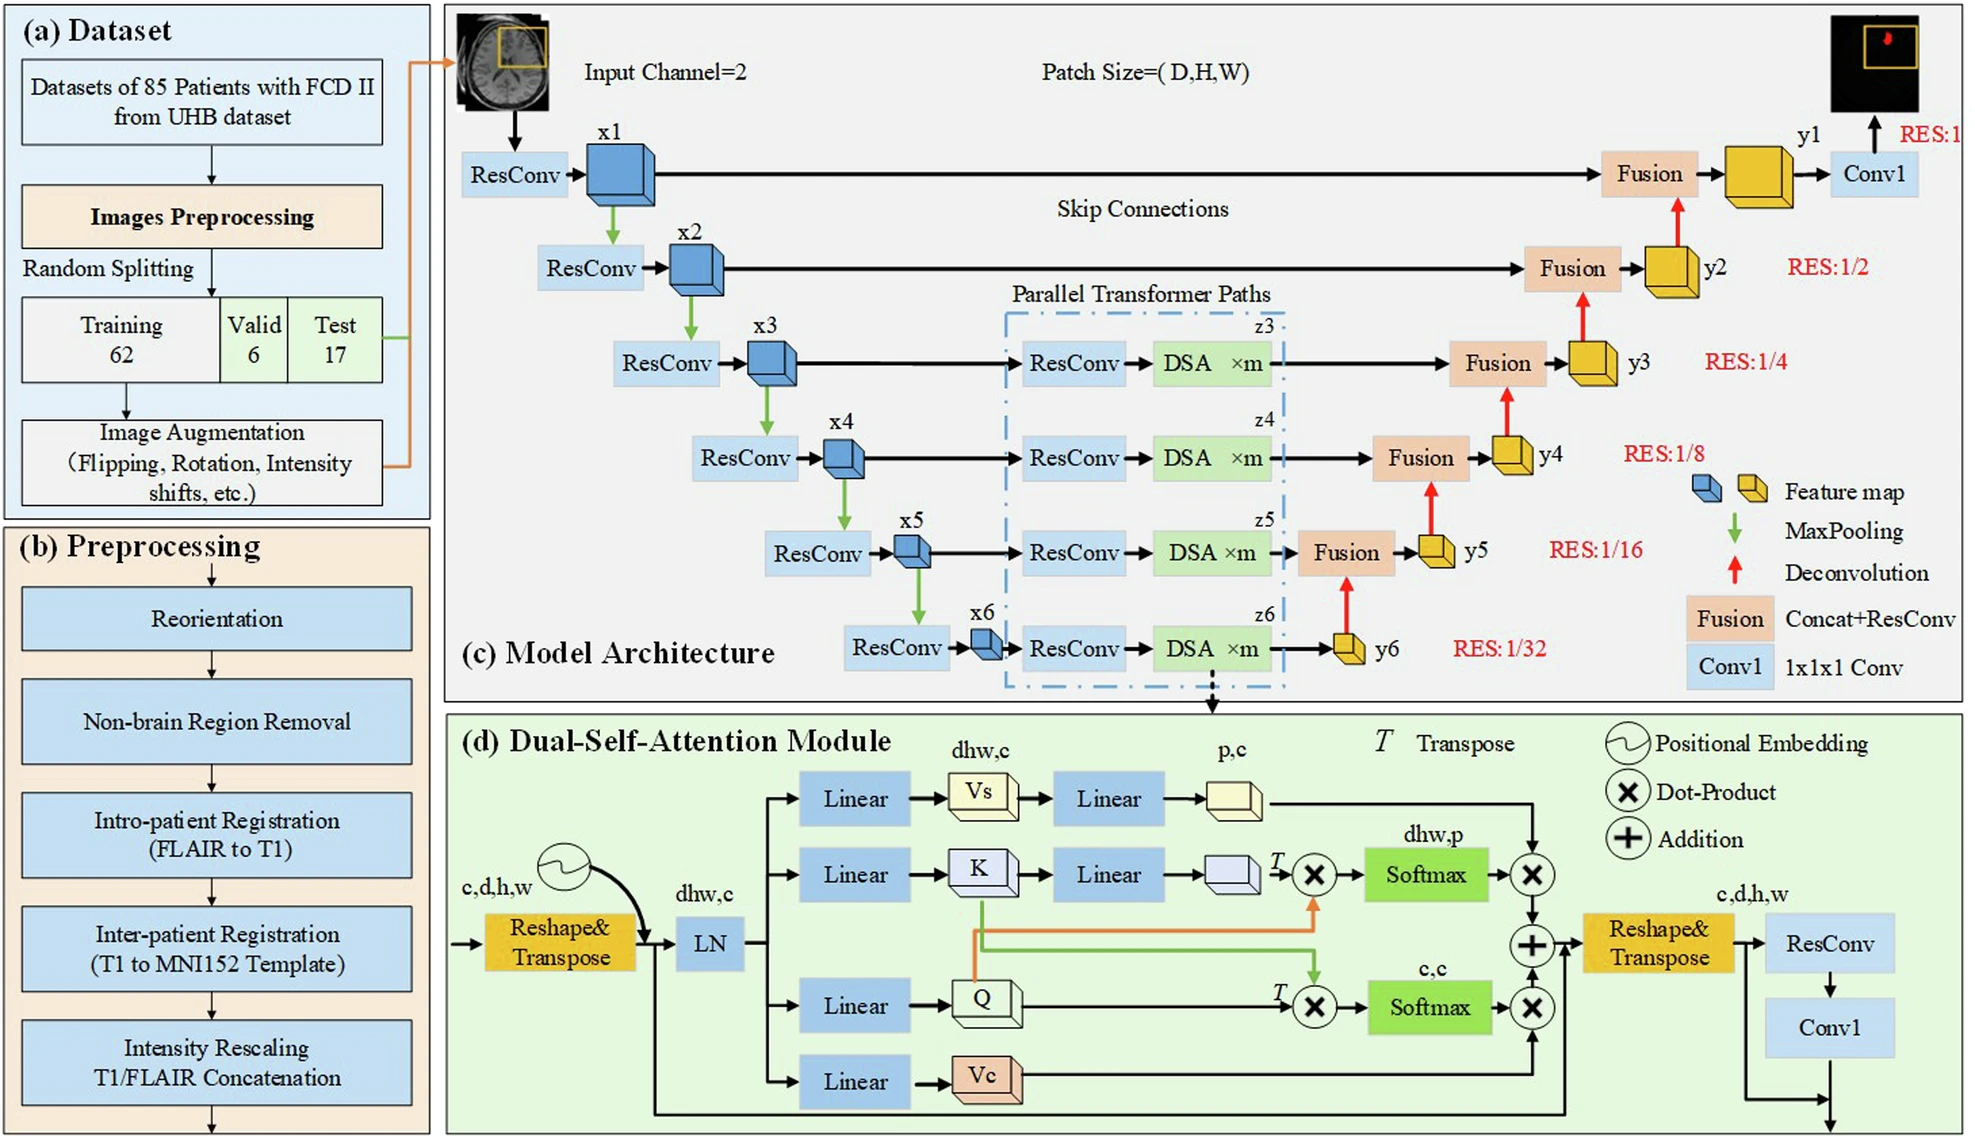
\includegraphics[width=\textwidth]{unet.png}
	\caption{a. Dataset splitting; b. Preprocessing procedure; c. Architecture of the proposed model based on an encoder-decoder structure. Parallel transformer pathways, each consisting of m dual-self-attention (DSA) modules, are inserted to capture the global features on feature maps of different resolutions, ranging from 1/4 to 1/32. d. Architecture of the DSA module, consisting of a spatial self-attention branch and a channel self-attention branch From research: \citeref{sub:sec:res8}}
	\label{fig:res8}
\end{figure}

\subsubsection{Results}

Here: \citeref{tab:res8}

\begin{table}[htbp]
	\centering
	\fbox{
	\begin{tabular}{l c}
		n & 170 \\
		patients & 85 \\
		controls & 85 \\
		train ratio & 0.6 \\
		test ratio & 0.25 \\
		valid ratio & 0.15 \\
	\end{tabular}
	}
	\caption{Benchmark}

	\fbox{
	\begin{tabular}{l c}
		Sensitivity & 82.4\% \\
		Specificity & ??\% \\
		Dice coefficient & 0.410
	\end{tabular}
	}
	\caption{Results from \citeref{sub:sec:res8}}
	\label{tab:res8}
\end{table}


\section{EEG-based DL/ML}

\subsection{\href{https://ieeexplore.ieee.org/abstract/document/7365453}{Epileptic Seizure Prediction Based on Multivariate Statistical Process Control of Heart Rate Variability Features (2016)}}

This one uses heart rate variability because: "Because excessive neuronal activities in the preictal period of epilepsy affect the autonomic nervous systems and autonomic nervous function affects HRV, it is assumed that a seizure can be predicted through monitoring HRV."

The goal is to have real-time prediction to improve their quality of live by alerting patients of seizures and 

\subsection{\href{https://dl.acm.org/doi/abs/10.1145/3386580}{Augmenting DL with Adversarial Training for Robust Prediction of Epilepsy Seizures (2020)}}

Using EEG, it wants to have real-time prediction. Paper not available freely.
